\documentclass{beamer}
\usepackage{graphicx}
\usepackage{amssymb}
\usepackage{amsmath}
\usepackage{bm}
\setbeamercovered{transparent}
\graphicspath{{../resources/}}

\title{Slides for Acemoglue Akcigit (2012)}
\author{Caleb Floyd and Tom Augspurger}
\date{\today}

\begin{document}

\frame{\titlepage}

% \section[Outline]{}
% \frame{\tableofcontents}

% Start with general intro to paper
% Then apply to software?
% Then compare to Boldrin Levine
% Probably skip the partial equilibrium intro?

% 1. What is the question this paper answers?
% 2. What was the state of knowledge before this paper?
% 3. How does this paper answer the question differently?
% 4. What are the main findings?

\section{Introduction}
\label{sec:introduction}

\begin{frame}[t]\frametitle{Intro}
  \begin{itemize}
    \item<+-> Dynamic environment to study optimal \emph{state-dependent} Intellectual Property Rights policy.
    \item<+-> IPR depends on technology gap in an industry (state-dependence).
    \item<+-> Tradeoff between monopolies and motivation for leaders.
  \end{itemize}
\end{frame}

\section{Literature Review}
\label{sec:literature_review}
\begin{frame}[t]\frametitle{Previous Research} 
  \begin{itemize}
    \item<+-> \emph{Static} tradeoff between R\&D incentive and monopoly distortions.
    \item<+-> Mechanism design approach.  Menu of patents and fees.
    \item<+-> Step-by-step innovation (Aghion, Harris and Vickers 1997) --- Higher growth from stiffer competition.
    \item<+-> Tournaments / Races
    %\item<+-> Look for predecessors of state-dependent IPR.  They claim to ``explicitly introduce'' it.
    %\item<+-> Look for predecessor of dynamic effects, not just static R\&D incentives / monopoly rents tradeoff.
    %\item<+-> Par. 3 pg. 5 notes some mechanism-design papers that might be worth skimming for previous research.
  \end{itemize}  
\end{frame}

\section{Contributions}
\label{sec:contributions}

\begin{frame}[t]\frametitle{New Contributions} 
  \begin{itemize}
    \item<+-> State-dependent IPR.
    \item<+-> Slow catch-up, compulsory licensing %(check on this).
    \item<+-> Full GE model % (probably done before, but first in the Aghion et. al line?)
  \end{itemize}
\end{frame}

\section{Model}
\label{sec:model}

\subsection{Preferences}
\label{sub:preferences}

\begin{frame}[t]\frametitle{Consumers' Preferences} 
  Single final good.  Continuum of 1 individuals.
  \begin{equation*} \label{eq:pref}
    \mathbb{E}_t \int_t^\infty exp(-\rho(s - t))\mathrm{ln}\,   C(s)ds
  \end{equation*}
  where $\rho$ is the discount factor.
  
  Also supply 1 unit of labor inelastically. 
\end{frame}

\subsection{Production}
\label{sub:production}

\begin{frame}[t]\frametitle{Technology-Final Good} 
  \begin{itemize}
    \item<+-> Output of final good: $Y(t) = C(t)$.
    
    \item<+-> Production of $Y(t)$:
      \begin{equation} \label{eq:tech_output}
        % Why log output? Cobb-Douglas since log of products is sum
        % i.e. the integral?  CD need not be HOD 1.
        \ln Y(t) = \int_{0}^{1} \ln y(j, t) d\,j 
      \end{equation}
      where $y(j, t)$ is the output of intermediate good $j$.
    
    %% Is this the right place for EE? 
    % \item<+-> Euler Equation:
    %   \begin{equation*}
    %     g(t) \equiv \frac{\dot{C}(t)}{C(t)} = \frac{\dot{Y}(t)}{Y(t)} = r(t) - \rho
    %   \end{equation*}
  \end{itemize}
\end{frame}

\begin{frame}[t]\frametitle{Technology-Intermediate Good} 
  \begin{itemize}
    \item<+-> $i$ denotes the firm.  Each industry $j \in [0, 1]$ has two firms competing.

    \item<+-> Intermediate goods produced according to:
      \begin{equation*} \label{eq:intermediate_production}
        y(j, t) = q_i(j, t)l_i(j, t)
      \end{equation*}
      where $q_i$ is a technology level and $l_i$ is labor used. 

    \item<+-> Yields marginal cost:
      \begin{equation*} \label{eq:marginal_cost}
        MC_i(j, t) = \frac{w(t)}{q_i(j, t)}
      \end{equation*}

    \item<+-> Limit pricing:
      \begin{equation*} \label{eq:limit_pricing}
        p(j, t) = \frac{w(t)}{q_{-i}(j, t)}      
      \end{equation*}
    where $-i$ denotes the follower (less advanced technology).
    \item<+-> Cobb-Douglas production of final good implies:
    %  TODO: Verify this.
      \begin{equation}
        y(j, t) = \frac{q_{-i}(j, t)}{w(t)}Y(t)
      \end{equation}
  \end{itemize}
\end{frame}

\begin{frame}[t]\frametitle{Technology-Innovation} 
  \begin{itemize}
    \item<+-> Innovation follows Poisson process with flow rate:
      \begin{equation} \label{eq:tech_rd_technology}
        x_i(j, t) = F(h_i(j, t))
      \end{equation}
      where $h_i(j, t)$ is the number of workers employed in R\&D.
      Also define $G(x_i(j,t)) \equiv F^{-1}(x_i(j,t))$ (R\&D employment).
    \item<+-> Successful innovation by the leader increments technology by factor $\lambda$.
    \item<+-> If the follower innovates, he catches up with the leader (Not patent infringing).
    \item<+-> Technology levels are ladder rungs: $q_i(j, t) = \lambda^{n_{ij}(t)}$, with $n_{ij}(t)$ giving the rung for firm $i$ in industry $j$.
    \item<+-> Mainly concerned with the technology gap: $n_j(t) = n_{ij}(t) - n_{-ij}(t)$
  \end{itemize}
\end{frame}

\subsection{Patent Policy}
\label{sub:patent_policy}

\begin{frame}[t]\frametitle{Patent Policy}
  \begin{itemize}
    \item<+-> Patents expire at Poisson rate: $\eta_{n_j}(t)$
    \item<+-> Preserves stationarity of the value functions.
    \item<+-> Law of motion for technology gap in industry $j$:
      \begin{equation*} \label{eq:tech_law_of_motion}
        \eta_j(t + \Delta t) =
        \begin{cases}
          \eta_j(t) + 1 & \textrm{prob } x_i(j,t)\Delta t + o(\Delta t)\\
          0 & \textrm{prob } x_{-i}(j,t)\Delta t + \eta_{n_{j(t)}}\Delta t + o(\Delta t) \\
          \eta_j(t) & \textrm{with the remainder} 
        \end{cases}
      \end{equation*}
  \end{itemize}
\end{frame}

% \subsection{Profits}
% \label{sub:profits}



\subsection{Equilibrium}
\label{sub:equilibrium}
\begin{frame}[t]\frametitle{Equilibrium} 

  $\bm{\mu}(t) \equiv {\mu_n(t)}_{n=0}^\infty$ is a distribution of \emph{industries} over \emph{technology gaps}.
  

\end{frame}

\begin{frame}[t]\frametitle{Labor Market} 
  \begin{itemize}
    \item<+-> Three sources of demand: Production of intermediaries, and R\&D by each firm.
    \item<+-> Combine demand for intermediates: $y(j, t) = q_i(j, t)l_i(j, t)$, and $y(j, t) = \frac{q_{-i}(j, t)}{w(t)}Y(t)$ to get

      \begin{equation}
        l_n(t) = \frac{\lambda^{-n}Y(t)}{w(t)}
      \end{equation}
    and so
      \begin{equation} \label{eq:labor_clearing}
        1 \geq \sum_{n=0}^{\infty} \mu_n(t) \Big[\frac{1}{\omega(t)\lambda^n} + G(x_n(t))    + G(x_{-n}(t))\Big]
      \end{equation}
      where $\omega(t)$ is labor's share of income.

  \end{itemize}
\end{frame}
\subsection{Steady State}
\label{sub:steady_state}
\begin{frame}[t]\frametitle{Firm's Value Function} 
  \begin{itemize}
    \item<+-> Net present value when leading by $n$:
      \begin{equation*}
        V_n(t) = \mathbb{E}_t \int_{t}^{\infty} exp(-r(s - t))[\Pi(s) - w(s)G(\hat{x}(s))]\,ds 
      \end{equation*}
    \item<+-> As a ``normalized''value function ($v_n(t) = V_n(t) / Y(t)$):
      \begin{equation*} \label{eq:rvf_leader}  % rvf: recursive value function
          pv_n = \max_{x_n \geq 0}\ \ (1 - \lambda^{-n}) - \omega^*G(x_n) + x_n[v_{n+1} - v_n] + [x_{-n}^* + \eta_n][v_0 - v_n]
        \end{equation*}
    \item<+-> Instantaneous operating profits: $(1 - \lambda^{-n})$.
    \item<+-> R\&D costs: $\omega^*(t)G(x_n(t))$.
    \item<+-> With probability $x_n(t)$ you innovate.
    \item<+-> With probability $x_{-n}^*(t) + \eta_n$ he innovates or your patent expires.
  \end{itemize}
\end{frame}

\begin{frame}[t]\frametitle{Firm's Value Function} 
  \begin{itemize}
    \item<+-> Tied firms value function:
      \begin{equation*} \label{eq:rvf_tied}
        \rho v_0 = \max_{x_0 \geq 0} -\omega^*G(x_{0}) + x_{0}[v_1 - v_0] + x_0^*[v_{1} - v_0]
      \end{equation*}

    \item<+-> Follower's value function:
      \begin{equation*} \label{eq:rvf_follower}
        \rho v_{-n} \max_{x_-n \geq 0} -\omega^*G(x_{-n} + [x_{-n} + \eta_n][v_0 - v_{-n}] + x_n^*[v_{-n-1} - v_{-n}])
      \end{equation*}
  \end{itemize}
\end{frame}

\begin{frame}[t]\frametitle{Optimization} 
  In equilibrium, R\&D poilcies must follow:
  \begin{align*} \label{eq:ss_rd_policies}
    x_n^*    &= max \big\{G'^{-1}\Bigg(\frac{[v_{n+1} - v_n]}{\omega^*}\Bigg)   ,0\}\\
    x_{-n}^* &= max \big\{G'^{-1}\Bigg(\frac{[v_0  - v_{-n}]}{\omega^*}\Bigg)   ,0\}\\
    x_0^*    &= max \big\{G'^{-1}\Bigg(\frac{[v_1     - v_0]}{\omega^*}\Bigg)   ,0\}
  \end{align*}

  Relationship between $v_n$ and $x_n$: Say patent protection weakens:
  \begin{itemize}
    \item<+-> Disincentive Effect: $\downarrow v_{n+1} \Rightarrow \downarrow v_{n+1} - v_n \Rightarrow \downarrow x_n^*$.
    \item<+-> Incentive Effect: $\downarrow v_{n+1} \Rightarrow \uparrow v_{n+2} - v_{n+1} \Rightarrow \uparrow x_{n+1}^*$.
    \item<+-> Composition Effect: $x_n$ is decreasing in $n$. More firms in close competition. Higher aggregate R\&D.
    \item<+-> Level Effect: Reduce prices and markups.  Less duplicative R\&D.
  \end{itemize}
\end{frame}

\section{Results}
\label{sec:results}
\begin{frame}[t]\frametitle{Uniform Policy} 
Problem is identical for all followers.

Given some assumptions (positive R\&D, non-zero profits) \ldots
\begin{itemize}
  \item<+-> $v_{-1} \leq v_0$; $\{v_n\}_{n=0}^{\infty}$ is bounded and strictly increasing.
  \item<+-> $x_0^* > x_1^*, x_0^* \geq x_{-1}^*$, and $x_{n+1}^* \leq x_n^*\ \forall n \in \mathbb{N}$.
\end{itemize}
\end{frame}

\section{Optimal IPR}
\label{sec:optimal_ipr}
\subsection{Benchmark: Full IPR}
\label{sub:benchmark_full_ipr}
\begin{frame}[t]\frametitle{Optimal Uniform IPR} 
  \begin{itemize}
    \item<+-> Turns out that if $\eta_n = \eta \ \forall n$, $\eta^* = 0$ (Patents never expire).
    \item<+-> Positive composition effect (more firms in close competition) overwhelmed by negative disincentive effect.
  \end{itemize}
\end{frame}

\begin{frame}[t]\frametitle{Optimal State-Dependent IPR} 
  \begin{itemize}
    \item<+-> Growth rate increases from 1.86\% to 2.04\%.
    \item<+-> Optimal patent length is increasing in technology gap. 
  \end{itemize}
\end{frame}

\begin{frame}[t]\frametitle{Full IPR} 
  \begin{center}
    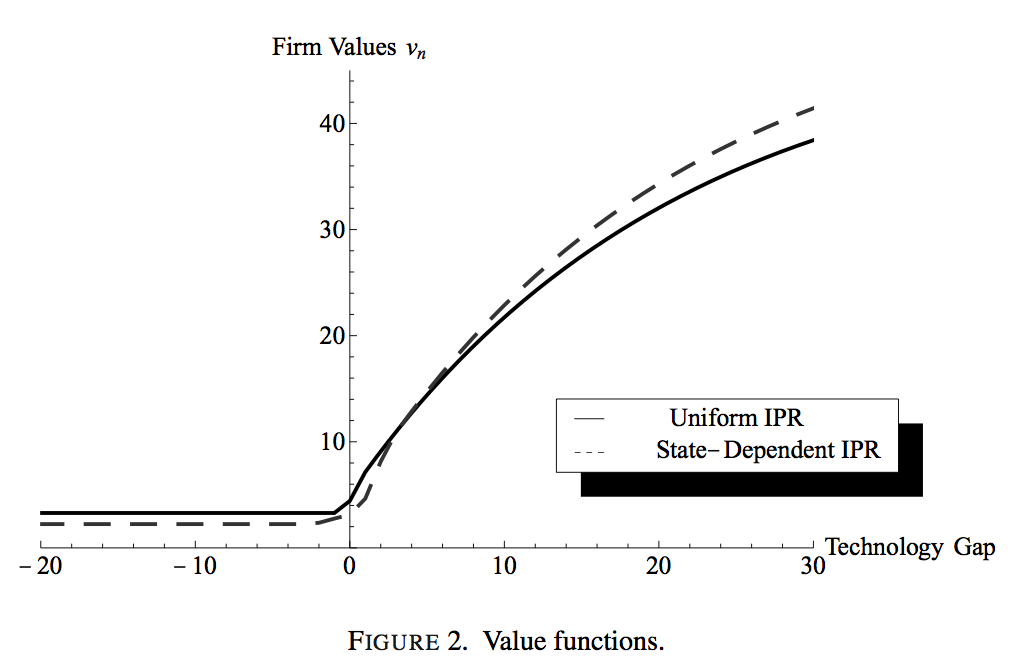
\includegraphics[scale=.31]{full_ipr_value.png}
    \label{fig:full_ipr}
  \end{center}
\end{frame}

\begin{frame}[t]\frametitle{Full IPR} 
  \begin{center}
    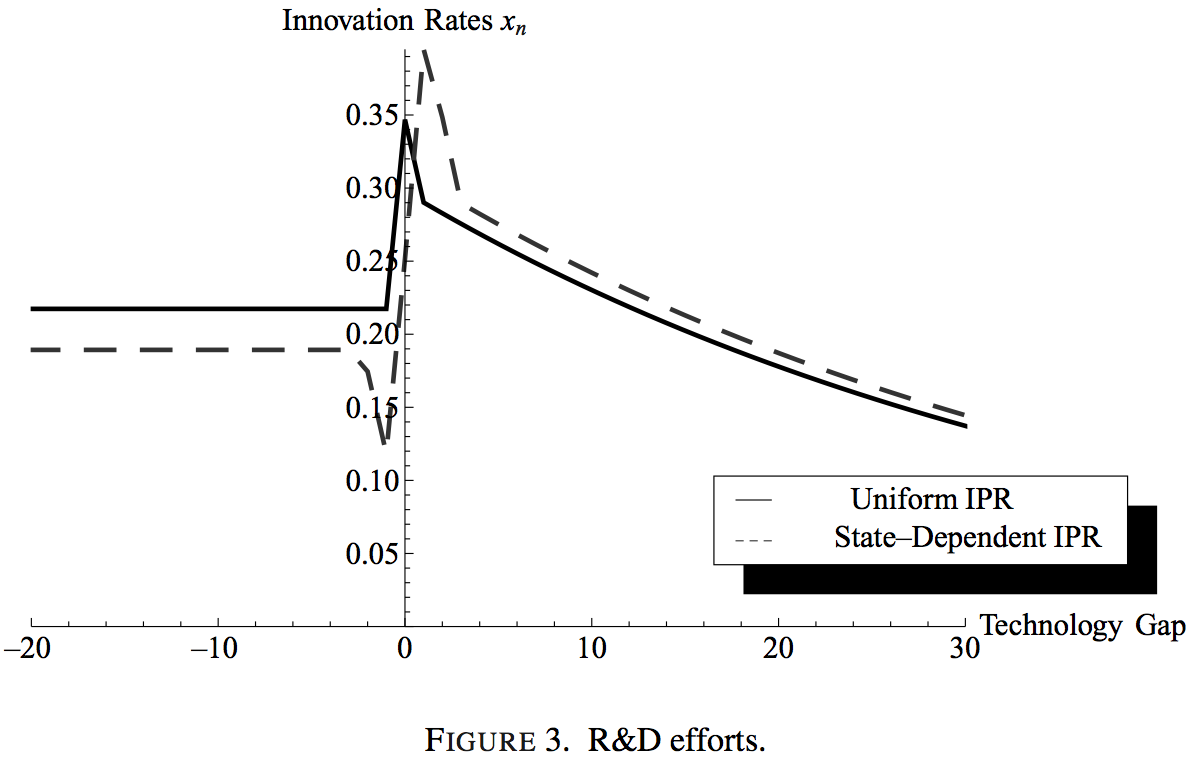
\includegraphics[scale=.28]{full_ipr_rnd.png}
    \label{fig:full_ipr}
  \end{center}
\end{frame}

\begin{frame}[t]\frametitle{Full IPR} 
  \begin{center}
    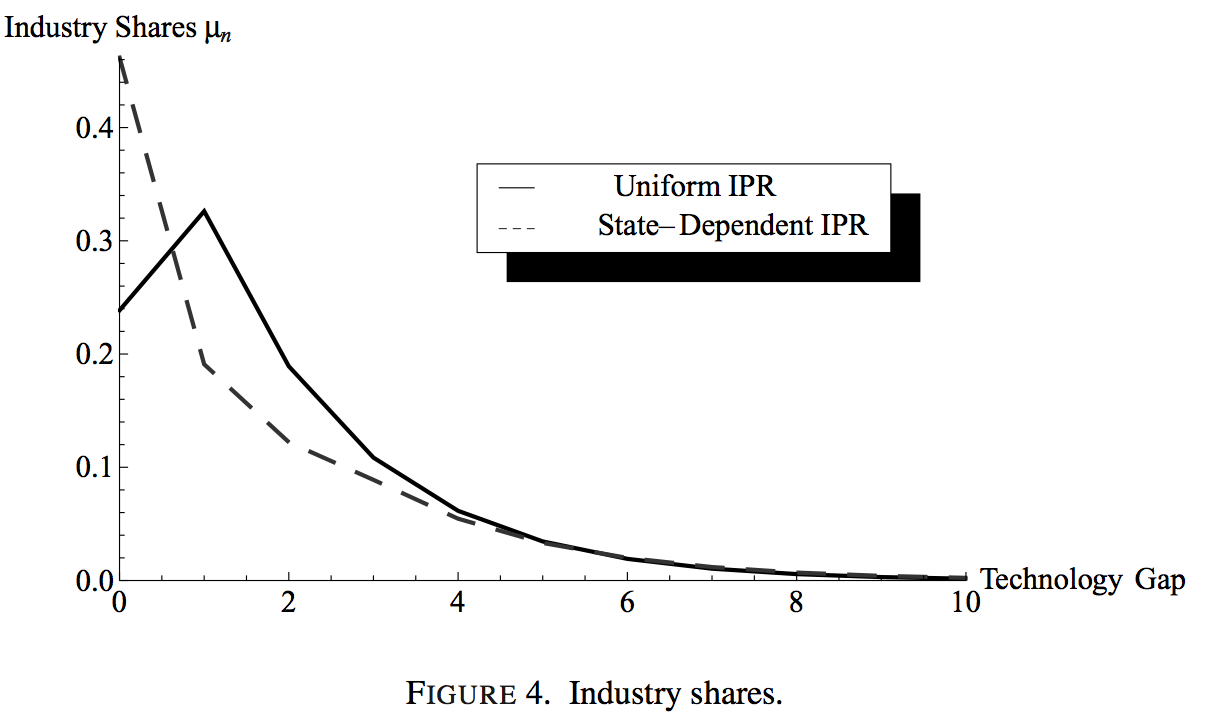
\includegraphics[scale=.28]{full_ipr_distbn.png}
    \label{fig:full_ipr}
  \end{center}
\end{frame}


\section{Software}
\label{sec:software}

\section{Summary}
\label{sec:summary}


\end{document}
